\begin{justify}
\glsreset{sf}
\chapter[Estado del arte]{Estado del arte}
\label{ch:estadodelarte}

En los últimos años, se ha generado un gran interés por el estudio sobre las tecnologías \gls{lpwan}, dado que son capaces de transmitir datos de forma inalámbrica a grandes distancias (las que en algunos casos alcanzan los \SI{15}{\kilo\meter}), pero a una baja tasa de transmisión de datos. Este tipo de tecnología inalámbrica provee un sinfín de aplicaciones posibles, y dada su gran versatilidad y autonomía puede ser usado desde el área de la medicina, como hasta en el sector agrario para control de cosechas. Estas características junto a la capacidad de transmisión y autonomía de estos dispositivos, ha llamado la atención de muchos investigadores, quienes se han dedicado a demostrar tanto las capacidades de los LoRa, como los límites de estas. Entregando así bastante información sobre su comportamiento físico y lógico, junto a la comprobación del cumplimiento y/o superación de las especificaciones técnicas publicadas por los fabricantes. Adicionalmente, se han realizado investigaciones sobre la integración del \gls{iot} en los dispositivos LoRa con el fin de realizar una mayor integración de soluciones inteligentes que pueden desarrollarse sobre la base de los \gls{lorawan}. Bajo este contexto, ha nacido la necesidad de un ambiente virtual para la utilización de estos dispositivos, donde algunos investigadores han realizado avances en el modelado de redes ALOHA bajo la utilización de software de simulación de eventos discretos, con el fin de poder reducir los costos asociados a la investigación junto a facilitar un medio portátil  para el estudio de estos dispositivos.\newpage \noindent
Los estudios que abarcan estos avances aquí expuestos se dividen en los siguientes temas:
\begin{itemize}
\item Funcionamiento de los dispositivos LoRA.\\
\item Limitaciones en el uso de \gls{lorawan}.\\
\item Modelado de redes ALOHA.\\
\item Integración de \gls{iot} en \gls{lorawan}.\\
\item Métodos de programación en C orientado a redes.\\
\end{itemize} 

\section{Funcionamiento de los dispositivos LoRa}
Los dispositivos LoRa son dispositivos diseñados para la comunicación inalámbrica a largas distancias basados en el antiguo protocolo ALOHA. Esta tecnología permite conectar dispositivos a una distancia de \SI{15}{\kilo\meter} en zonas suburbanas, y hasta \SI{2}{\kilo\meter} en zonas urbanas \cite{Sornin}~\cite{Sornin2}. Además estos poseen una autonomía mucho mayor dado que utilizan un método optimizado de asignación de ventanas de tiempo para la transmisión, basado en su predecesor ALOHA en su variante Slotted, el que se caracteriza por generar un sistema de programación de mensajes desde el \textit{gateway} a sus nodos, donde se asignan ventanas de transmisión por fracciones de tiempo, minimizando de esta forma las colisiones de paquetes entre nodos~\cite{NORMAN}. Los nodos, en caso de no poseer activas ventanas de transmisión, estos se colocan en estado de hibernación o reposo, hasta que llega el segundo de transmitir datos al \textit{gateway}. Adicionalmente se expone, que \gls{lorawan} implementa un manejo de múltiples canales en base a espectros de señal, los que poseen una diferencia tal en su frecuencia, que no poseen interferencia entre ellos \cite{modulation}. Cada una de estas diferenciales de frecuencia usadas del espectro expandido son denominadas \gls{sf}, donde es asignado un identificador a cada banda de frecuencia disponible por cada canal de comunicación. Esta técnica llamada \textit{Spreading Spectrum} permite que las comunicaciones de \gls{lorawan} posean una mayor resistencia frente a interferencias de medios externos, el operar con una baja densidad espectral de energía, como también el otorgar un canal seguro de comunicación, no permitiendo el acceso a oyentes no autorizados, ya que es imperante conocer la frecuencia base de la señal para poder decodificarla. Asimismo cada canal posee una determinada ganancia de la velocidad de transmisión a cambio de la disminución de la distancia de transmisión y viceversa, esto es posible mediante el uso de métodos de \gls{adr}. El \textit{gateway} LoRa asigna un \gls{sf} o una lista de canales disponibles en caso de ser posible, para que el nodo pueda comunicarse con el \textit{gateway}.\\
Las especificaciones aquí expuestas, son utilizadas para este proyecto de título, para poder comprender el comportamiento, tanto lógico, como físico de los dispositivos \gls{lorawan}, con el fin último de poder modelar estos comportamientos con una herramienta de simulación de redes y lograr una simulación análoga al comportamiento de los dispositivos LoRa en el ámbito físico y lógico.

\section{Limitaciones en el uso de LoRaWAN}
Los dispositivos LoRa poseen dentro de sus especificaciones técnicas, la definición de parámetros que determinan a la larga el comportamiento de estos artefactos, como por ejemplo la distancia máxima de transmisión, las bandas de frecuencia en las que trabaja, entre otros~\cite{orange}. Estas capacidades han sido puestas a prueba para conocer los límites de las capacidades de \gls{lorawan}~\cite{Xavier}. Dentro de los ámbitos verificados, está la limitación de la capacidad del canal y el máximo tamaño de una red LoRa (sobre la base del número de nodos y \textit{gateways} en la red). Como aporte de este artículo, está la definición de la diferencia real entre las tasas de transmisión, entre los diferentes \gls{sf}, tomando en cuenta el tiempo que toma el paquete en viajar en el aire hacia su destino (\textit{Time on Air}), como también el tamaño del \textit{payload}~\cite{Xavier}. Estas diferencias pueden apreciarse en la Fig~\ref{arte:1}, donde al usar un \gls{sf} que posee menor alcance de transmisión efectiva, es posible notar una transmisión más expedita del \textit{payload} enviado, aún así, a tamaños mayores de \textit{payload}, en los \gls{sf} de mayor alcance de transmisión, el tiempo de viaje a destino es mucho mayor que en el resto de \gls{sf} de menor alcance. Adicionalmente, los investigadores indican que el desempeño de una red LoRa, depende de la fracción de tiempo en que el canal está ocupado (\textit{Duty Cycle}), y de las colisiones inherentes de un enlace basado en el protocolo ALOHA, como puede verse en la Fig~\ref{arte:2} al aumentar el número de nodos LoRa (representado con N en el gráfico), disminuye considerablemente la cantidad de paquetes recibidos, esto en parte se debe a la saturación del canal producida por colisiones de paquetes enviados al \textit{gateway}, junto con las retransmisiones provenientes de los nodos, que terminan por amplificar el efecto de las colisiones iniciales produciendo una saturación del canal. Esta saturación del canal ocurre por cómo está diseñada la transmisión y retransmisión de paquetes del protocolo ALOHA, donde si un paquete es enviado, y en un tiempo determinado el nodo no recibe un acuse de recibo del paquete enviado, este transmitirá en la siguiente ventana disponible de tiempo el mismo paquete hasta que reciba una respuesta~\cite{NORMAN}. El problema es que al aumentar el número de nodos las ventanas de tiempo, disminuyen tanto en número, cómo en duración de éstas, por lo que es más frecuente las colisiones dentro de éstas.\\
\begin{figure}[!b]
\centering
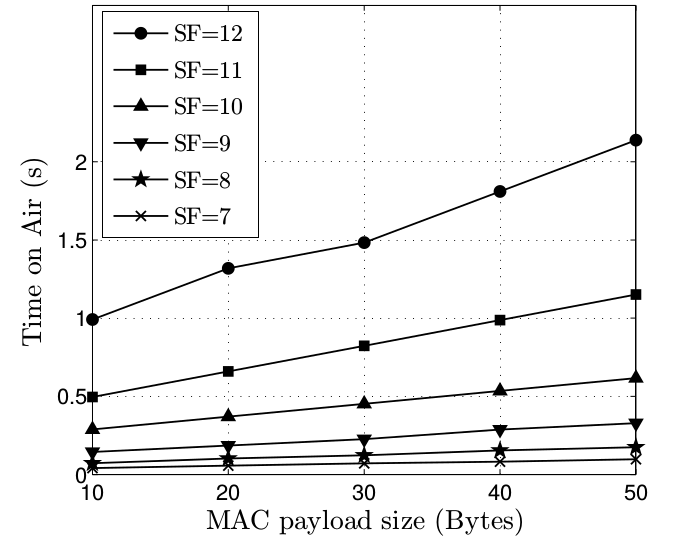
\includegraphics[scale=0.4]{images/estadoarte1.png}
\caption{Gráfica de tamaño de \textit{payload} MAC por tiempo que toma el paquete en llegar a destino. Fuente:\cite{Xavier}}
\label{arte:1}
\end{figure}
\begin{figure}[!ht]
\centering
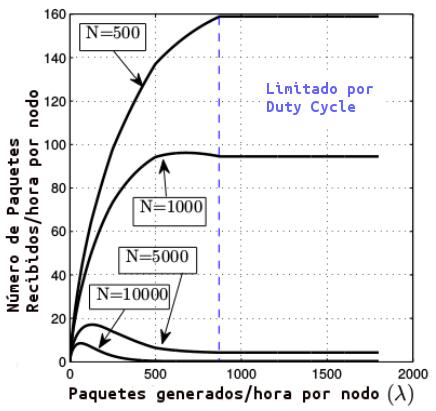
\includegraphics[scale=0.5]{images/estadoarte2.png}
\caption{Gráfica de paquetes generados en una hora por número de paquetes recibidos en una hora. Fuente:\cite{Xavier}}
\label{arte:2}
\end{figure}
Por otra parte, en otra investigación, se colocaron a prueba las capacidades de transmisión, pero en relación a la distancia máxima de transmisión, en zonas llanas sin interferencia por edificios o personas, y en zonas urbanas, con el objetivo de determinar si los LoRa cumplen con las especificaciones que entregan, y por otra parte, averiguar si pueden sobrepasar estas especificaciones técnicas entregadas por los fabricantes y descubrir nuevos límites para el uso de los dispositivos LoRa~\cite{Juha}.\\
En relación a las pruebas realizadas, el \textit{gateway} es situado a \SI{24}{\meter} sobre la altura del mar con una antena bi-cónica de \SI{2}{dbi} de ganancia, donde los nodos con los que se comunicará, uno estará navegando sobre un bote en un ambiente libre de edificios y árboles, mientras que el otro estará sobre el techo de un automóvil, donde cada nodo se alejará cada vez más sobre su medio de transporte, para evaluar si es posible transmitir efectivamente dentro de los parámetros que indican los fabricantes de LoRa, o si incluso es posible superar estas especificaciones. Los resultados obtenidos de las pruebas de medición de la investigación, pueden verse en las Tab~\ref{arte:3} y Tab~\ref{arte:4}~\cite{Juha}.\\
\begin{table}[!ht]
\centering
\begin{tabular}{|c|c|c|c|}
\hline
Rango & Número de            & Número de          & Porcentaje de  \\
      & paquetes trasmitidos & paquetes recibidos &  pérdida\\ 
      &                      &                    &   de paquetes \\ \hline
\si{0-2}{km} & \num{894} & \num{788} & \SI{12}{\percent} \\ \hline
\si{2-5}{km} & \num{1215} & \num{1030} & \SI{15}{\percent} \\ \hline
\si{5-10}{km} & \num{3898} & \num{2625} & \SI{33}{\percent} \\ \hline
\si{10-15}{km} & \num{932} & \num{238} & \SI{74}{\percent} \\ \hline
Total & \num{6813} & \num{4506} & \SI{34}{\percent} \\ \hline
\end{tabular}
\caption{Cantidad de paquetes transmitidos, recibidos y pérdida de paquetes por rango de distancia en medición hecha por nodo sobre auto. Fuente:\cite{Juha}}
\label{arte:3}
\end{table}

\begin{table}[!ht]
\centering
\begin{tabular}{|c|c|c|c|}
\hline
Rango & Número de            & Número de          & Porcentaje de  \\
      & paquetes trasmitidos & paquetes recibidos &  pérdida\\ 
      &                      &                    &   de paquetes \\ \hline
\si{5-15}{km} & \num{2998} & \num{2076} & \SI{31}{\percent} \\ \hline
\si{15-30}{km} & \num{690} & \num{430} & \SI{38}{\percent} \\ \hline
Total & \num{3688} & \num{2506} & \SI{32}{\percent} \\ \hline
\end{tabular}
\caption{Cantidad de paquetes transmitidos, recibidos y pérdida de paquetes por rango de distancia en medición hecha por nodo sobre bote. Fuente:\cite{Juha}}
\label{arte:4}
\end{table}
\newpage \noindent
Los resultados obtenidos a través de esta investigación, son de gran ayuda para el desarrollo de este proyecto, dado que entrega una guía de valores esperados al momento de realizar mediciones con los dispositivos reales~\cite{Juha}. Asimismo, otorga una guía de como se manifiestan parámetros como la tasa de errores en paquetes \gls{per}, para luego integrar al simulador con el fin de acercarlo más al funcionamiento real de los dispositivos. Y de la misma manera en la investigación que pone a prueba las capacidades de LoRa, entrega los conocimientos suficientes para poder modelar el comportamiento real de la saturación del canal en base a las retransmisiones de los nodos, y las colisiones generadas~\cite{Xavier}.
\section{Modelado de redes ALOHA}

El estándar \gls{lorawan} trabaja sobre la base del protocolo ALOHA, el cual es uno de los primeros protocolos de comunicación orientados a la conexión de dispositivos de forma inalámbrica. ALOHA trabaja sobre un canal de radio frecuencia, que utiliza tanto para el envío, como para la recepción de datos, por lo que para aumentar la transmisión efectiva de datos (\textit{throughput}), el protocolo ALOHA puro transmite datos en ventanas de tiempo aleatorias, y en caso de que el receptor no responda, en más del doble del tiempo que debiera responder con un acuse de recibo o \gls{ack}, el dispositivo emisor retransmitirá este paquete, y procederá con ese procedimiento hasta que reciba un acuse de recibo, con lo que concluye su transmisión de datos. Por otra parte Slotted ALOHA  o ``Ranurado'' implementa discretas ventanas de tiempo, donde el sólo podrá enviar o recibir datos, al inicio de una ventana de tiempo, con lo que se minimiza el número de colisiones~\cite{NORMAN}.\\
Slotted-ALOHA al ser un protocolo que permite las comunicaciones inalámbricas, con un buen manejo de colisiones, gracias a sus ventanas de tiempo discretas. Esta cualidad, llamó el interés de investigadores en generar ambientes virtuales, para simular el comportamiento de estos dispositivos, con el fin de poder realizar pruebas y estudios sobre el uso de este protocolo, sin necesidad de tener que instalar una red ALOHA con todos los costos asociados, tanto de tiempo como de dinero~\cite{Abdullah}.\\
En relación a los aportes del modelado de sistemas Slotted ALOHA, se realizan tres modelos que permiten el múltiple acceso de computadores mediante Slotted ALOHA, con el fin de otorgar modelos de simulación del protocolo para que estudiantes puedan comprender de mejor forma el cómo se comunican los dispositivos ALOHA~\cite{Abdullah}. Estos modelos de simulación imitan el comportamiento lógico del protocolo, entregando una herramienta útil para la comprensión del funcionamiento de redes de este tipo. Bajo este contexto, de la misma forma que nació la necesidad de modelar el funcionamiento del protocolo ALOHA. Adicionalmente se realizaron avances en el modelado de redes de sensores a gran escala, lo que entrega modelos que describen no sólo el funcionamiento del protocolo en condiciones ideales, si no que también la capacidad de modelar condiciones de borde y situaciones diferentes de las ideales, lo que acerca al módelo, a un comportamiento análogo al presente en los dispositivos reales~\cite{simulato}~\cite{simubook}.\\
Por otra parte, en una investigación se entrega un estudio sobre los diferentes simuladores de redes que existen, sus ventajas y desventajas frente al resto y los protocolos que acepta cada una de estas herramientas computacionales y sobre las capacidades de integración entre protocolos y tecnologías que ofrecen los distintos conjuntos de herramientas de simulación (\textit{frameworks})~\cite{Murat}.\\
En relación con este proyecto, todas las investigaciones mencionadas en este apartado, entregan la base teórica para el entendimiento del protocolo ALOHA, el cual es la base del funcionamiento de los dispositivos LoRa, y junto a esto hay investigaciones que entregan técnicas y métodos de cómo modelar tanto funcionamiento ideal y comportamiento lógico de protocolos en base a máquinas de estado ( en el caso de una simulación de eventos discretos), como también sobre el modelado de redes con parámetros como \gls{per}, atenuación de señal, entre otros elementos, que permiten el acercar un modelo de simulación, al comportamiento análogo de dispositivos reales~\cite{Abdullah}~\cite{simulato}. Cabe destacar que hay un artículo, que aporta con información sobre los diferentes \textit{frameworks} de simulación de redes, lo que permite tener una cantidad aceptable de información para poder decidir que software utilizar a la hora de desarrollar el simulador de dispositivos LoRa~\cite{Murat}.

\section{Integración de IoT en LoRaWAN}

%%tesis tomas, header compression y aplicaciones iot de lora%%
Los dispositivos LoRa, se comunican en base a transmisión de datos por radio frecuencia de un salto, esto junto con sistemas de modulación LoRa. En el escenario de enviar los datos obtenidos por los nodos LoRa con una aplicación web, el sistema no podría enviar los datos a través de Internet dado que no posee la capacidad de enrutamiento, no obstante el \textit{gateway} LoRa es capaz de realizar una retransmisión de los paquetes recibidos hacia un \textit{backend} (computador remoto) y con esto permitir la conectividad con aplicaciones web para la recepción de datos, aunque hasta el momento no es posible saber que nodo mandó un dato específico, o enviar datos desde el \textit{gateway} de forma directa hacia una dirección IP, esta carencia de los dispositivos LoRa limita las posibles aplicaciones con estos dispositivos. Bajo este contexto, algunos investigadores  han realizado modelos de compresión de cabeceras del protocolo IPv6 para dispositivos bajo el estándar \gls{lpwan}, donde se propone un modelo llamado 6LoWPAN que elimina ciertos campos de la cabecera del protocolo IPv6, de acuerdo a la configuración de los primeros \SI{16}{\bit}, con el fin de reducir el tamaño de la cabecera del paquete para direcciones IPv6 unicast, donde puede comprimirlos a \SI{512}{\bit} o \SI{128}{\bit} dependiendo de que campos se omiten, u omitir los campos opcionales por completo~\cite{lowpan}. En \cite{tomas}, este modelo teórico es aplicado a una red LoRa donde la cabecera IPv6 comprimida junto con el \textit{payload} deseado, se enviará a través del \textit{payload} de dispositivos \gls{lpwan} hacia el \textit{gateway}. Una vez llegado al \textit{gateway}, en este se construirá un paquete IPv6 con las especificaciones entregadas en la cabecera comprimida, donde adicionalmente se agregará la información relacionada al \textit{payload} del nodo emisor, y sus direcciones de red, las cuales al ser pertenecientes a una red LoRa, serán ingresadas en una tabla de enrutamiento que poseerá una equivalencia entre direcciones IPv6 y dirección de red LoRa, con el fin de poder luego enviar datos directamente desde los nodos hacia direcciones IPv6 y viceversa entregando la nueva función al \textit{gateway} LoRa de enrutador de mensajes.\newpage
\noindent
Cabe decir de que el \textit{gateway} LoRa para esta funcionalidad, necesita estar conectado al computador remoto que le provee de conexión a Internet, por medio de una interfaz virtual \gls{tun}, la que dejará pasar directamente los datos desde la red LoRa desde el \gls{tun} (donde está conectado el \textit{gateway} LoRa), hacia la salida a Internet del computador remoto. Si bien, la retransmisión de paquetes que posee nativa, realiza el mismo procedimiento, con la diferencia que ahora el \textit{gateway} LoRa creará el paquete de datos que se enviará, y este sólo será retransmitido hacia Internet, en cambio antes, el computador remoto tenía la labor de crear dicho paquete de datos, lo que entrega mayor autonomía e independencia de uso a los dispositivos LoRa.\\
Estos avances sobre la compresión de la cabecera IPv6 para dispositivos \gls{lpwan}, y la integración de IPv6 mediante el uso de estos modelos de compresión en una red LoRa, entregan a este proyecto el conocimiento necesario para poder diseñar un módulo que permita actuar de gestor de transición de una comunicación directa desde el \textit{gateway} hacia servicios locales dentro del computador remoto (sean bases de datos o aplicaciones web locales), y un intermediario mas seguro para la retransmisión de los paquetes, dado que al comunicarse directamente con la \gls{api} dentro del módulo bajo una conexión por \gls{socket}, entrega la posibilidad de realizar una conexión con un mayor nivel de seguridad, al tener la posibilidad de utilizar protocolos como TLS que dan la capacidad de cifrar la información y así evitar que un tercero atente contra la privacidad, integridad o disponibilidad de los datos.
\newpage
\section{Métodos de programación en C orientado a redes.}
%%libro de sockets, integracion de modulo%%
En muchas aplicaciones web, se han de utilizar scripts en sus servicios web para que realicen acciones deseadas por los desarrolladores, como también muchas veces son desarrollados scripts en el \textit{backend}, para realizar procedimientos como entrega de datos, creación de objetos, entre otros. El problema nace en que estos scripts son desarrollados en lenguajes como Python, Java o C, los que no tienen una orientación a red, si no, más bien a objetos, lo que dificulta el traspaso de datos obtenidos por los scripts hacia las aplicaciones web o sus servicios relacionados.\\
Bajo este contexto, nace la necesidad de que los scripts contenidos en aplicaciones web, se conecten tanto a \glspl{api} como a otros servicios existentes. Para poder llevar a cabo esta tarea, es necesario el uso de \glspl{socket}, los que constan de la apertura de conexiones bidireccionales a puertos determinados, que permiten la interacción en lectura como escritura contra servicios y aplicaciones web (Bases de datos, \glspl{api}, archivos de configuración, registros de depuración, etc). En el texto ``Programación en C orientada a redes'', enseñan múltiples técnicas, métodos y plantillas de código que permiten establecer conexión con servicios de red mediante el uso de \glspl{socket} en el lenguaje C~\cite{network}.\\
Los conocimientos aportados por este libro ayudaron en el desarrollo del módulo de transición de \gls{lorawan} a IPv6 en este proyecto, aportando métodos y funciones que otorgan la capacidad de conectar el \textit{gateway} LoRa con servicios y aplicaciones web. Esta conexión es generada en el mismo script que maneja la recepción de los mensajes de los nodos LoRa con el protocolo IPv6 integrado, resultando de esta forma, un sistema íntegro y con un nivel mayor de seguridad para poder conectar los datos obtenidos en la red LoRa con una aplicación web y todos sus servicios de red asociados.
\end{justify}